\documentclass[10pt,a4paper]{article}
\usepackage[a4paper,margin=21mm]{geometry}
\usepackage[T1]{fontenc}
\usepackage[utf8]{inputenc}
\usepackage{lmodern}
\usepackage{amsmath,amssymb,booktabs,graphicx,hyperref,xcolor,microtype}
\usepackage{enumitem}
\usepackage{float}
\usepackage{fancyhdr}
\usepackage[font=small,labelfont=bf]{caption}
\definecolor{navy}{HTML}{19324D}
\definecolor{teal}{HTML}{157F86}
\hypersetup{colorlinks=true,linkcolor=navy,urlcolor=teal,citecolor=navy}
\setlength{\parindent}{0pt}
\setlength{\parskip}{5pt}
\setlist[itemize]{topsep=2pt,itemsep=2pt,leftmargin=16pt}
\pagestyle{fancy}
\fancyhf{}
\lhead{\small\color{navy}CELL-FREE MIMO / GNN / REPRODUCIBILITY}
\rhead{\small\color{navy}NOVEMBER 2026}
\cfoot{\small\thepage}
\renewcommand{\headrulewidth}{0.4pt}
\newcommand{\sect}[1]{\vspace{3pt}\section{\color{navy}#1}}
\begin{document}
\begin{center}
{\small\color{teal}\textbf{INDEPENDENT REPRODUCIBLE TECHNICAL REPORT \;\textbullet\; v0.1}}\\[8pt]
{\LARGE\bfseries\color{navy}Graph-Based Downlink Power Allocation in\\[2pt] Cell-Free Massive MIMO}\par
\vspace{5pt}
{\large A Pilot Study Under AP Outages and CSI Perturbations}\par
\vspace{10pt}
{\bfseries Amirmohammad Goodarzy}\par
{\small Bachelor's student, University of Messina \;|\; Milan, Italy \;|\; 12 November 2026}\par
\vspace{5pt}
{\footnotesize \textit{Independent portfolio research; not peer reviewed, not published in a journal, and not an official University of Messina result.}}
\end{center}
\vspace{2pt}
\noindent\colorbox{navy!6}{\parbox{0.966\linewidth}{\small\textbf{Abstract.}\; We present a reproducible, small-scale computational study of fairness-oriented downlink power allocation in a simplified user-centric cell-free massive MIMO network. The simulator uses independent Rayleigh fading, orthogonal uplink pilots, normalized maximum-ratio precoding and a use-and-then-forget spectral-efficiency bound. A bipartite AP--UE graph neural network (GNN) is trained without target optimizer labels and compared against equal allocation, gain-proportional allocation and a per-instance iterative reference. On 192 independent synthetic test layouts with 16 access points (APs) and 4 users, mean worst-user spectral efficiency is \textbf{1.537 bit/s/Hz} for the GNN versus \textbf{1.274} for equal allocation and \textbf{1.565} for the non-certified iterative reference. Under a 25\% AP outage, the GNN obtains \textbf{1.268}; under a bounded white-box perturbation of reported large-scale fading, \textbf{1.472}. These are \emph{single-seed illustrative results}, not measurements of deployed 6G networks or claims of algorithmic novelty. Code, seeds, logs and plots are provided for reproduction.}}

\sect{Motivation and scope}
Cell-free massive MIMO distributes cooperating APs instead of assigning each device to an isolated cell. Its achievable rates depend on cooperation, channel estimation, precoding, association and power control. The foundations and modeling tradeoffs are established by Demir, Bj\"ornson and Sanguinetti~\cite{demir2021}. Prior work already investigates GNN-based power allocation in partially connected cell-free systems~\cite{mishra2024} and energy efficiency~\cite{raghunath2024}. \textbf{This report does not claim that GNN power control is new.} Its purpose is to demonstrate an auditable implementation and a controlled failure/CSI-error experiment suitable for a research internship portfolio.

The research questions are (Q1) can a small permutation-equivariant GNN improve worst-user rate relative to simple heuristic allocations? (Q2) how does its performance change under AP removal and input-channel estimation errors? (Q3) how closely does it track an inexpensive per-scenario gradient-based reference?

\sect{Simplified system and rate model}
We consider $M=16$ single-antenna APs serving $K=4$ single-antenna user equipments (UEs) in TDD. A user selects its $L=8$ strongest APs by large-scale fading. Let $\beta_{mk}$ denote the normalized large-scale gain of the AP--UE link and $h_{mk}\sim\mathcal{CN}(0,\beta_{mk})$ the small-scale channel. The AP association mask is $a_{mk}\in\{0,1\}$.

With independent Rayleigh fading, mutually orthogonal uplink pilots of length $\tau_p\geq K$, pilot power $p_p$, and noise $\sigma^2$, the channel-estimate variance is
\begin{equation}\label{eq:gamma}
\gamma_{mk}=\frac{\tau_p p_p\beta_{mk}^2}{\tau_p p_p\beta_{mk}+\sigma^2}.
\end{equation}
AP $m$ transmits $x_m=\sum_k\sqrt{p_{mk}}\,\widehat h_{mk}^{*}/\sqrt{\gamma_{mk}}\,s_k$ with normalized independent unit-power symbols $s_k$, and $p_{mk}=0$ when $a_{mk}=0$. The \emph{per-AP constraint} is $\sum_k p_{mk}\leq P_m$, with $P_m=1$ in this normalized experiment. The use-and-then-forget (UatF) lower bound for independent channels and orthogonal pilots gives
\begin{equation}\label{eq:sinr}
\mathrm{SINR}_k = \frac{\bigl(\sum_m\sqrt{p_{mk}\gamma_{mk}}\bigr)^2}
{\sum_m\beta_{mk}\sum_jp_{mj}+\sigma^2},\quad
\mathrm{SE}_k=\left(1-\frac{\tau_p}{\tau_c}\right)\log_2(1+\mathrm{SINR}_k).
\end{equation}
The denominator includes noncoherent beamforming uncertainty/inter-user interference; \emph{pilot contamination and coherent contamination terms are absent by assumption}. This is an analytical SE lower bound, not an instantaneous-rate simulator. We use $\tau_p=4$, $\tau_c=200$, $p_p=1$ and $\sigma^2=10^{-3}$.

\sect{Methods and data generation}
\textbf{Synthetic geometry.} Each layout samples AP and UE locations independently and uniformly within a $500\,$m $\times 500\,$m square. We use $\beta_{mk}=\min\{1,(50/\max(d_{mk},10))^{3.2}\}$, where distance is in metres. This is intentionally a \emph{normalized toy path-loss law}, not calibrated 3GPP propagation. Train, validation and test sets contain 480, 96 and 192 independent layouts (seeds 43, 44 and 45). No test-layout parameters are used during training or checkpoint selection.

\textbf{Policies.} The equal policy shares each active AP's power uniformly across connected users. The gain-proportional policy allocates a share proportional to the observed $\beta_{mk}$. The iterative reference optimizes masked AP-wise softmax logits using 125 Adam iterations on the same observed channel statistics; it is \emph{not a certified optimizer or global upper bound}. The learned policy is a two-round, width-32 bipartite message-passing GNN: shared edge MLPs exchange information through mean-aggregated AP/UE embeddings, after which AP-wise masked softmax transforms edge scores into feasible transmit power fractions. APs serving no users transmit zero. Its outputs are equivariant to permutations of AP and UE labels (a property tested in the repository).

\textbf{Training.} The network directly maximizes a differentiable soft minimum of modeled user rates,
\begin{equation}
\mathcal{J}(\theta)=\mathbb{E}\left[-T\log\sum_{k=1}^K\exp\big(-\mathrm{SE}_k(\theta)/T\big)\right],\qquad T=0.35,
\end{equation}
with Adam learning rate $2\times10^{-3}$, weight decay $10^{-5}$, batches of 48 and 80 epochs. The best held-out validation checkpoint occurred at epoch 77. \textbf{No optimizer-generated labels or test layouts} are used for GNN training.

\textbf{Stress tests.} We (i) independently disable 25\% of APs per test layout, applying the same removal mask to all methods; (ii) corrupt reported log-gains via independent uniform errors $\delta_{mk}\in[-0.3,0.3]$, so $\widetilde\beta_{mk}=\min(1,\beta_{mk}e^{\delta_{mk}})$; and (iii) compute a single-step white-box gradient perturbation of reported $\log\beta$ within the same magnitude limit, specifically \emph{targeted against the learned GNN}. Actual achievable rates are always evaluated on the \emph{true} $\beta$, and the association is kept fixed. This attack is a \emph{controller-feature threat model}, not radio-frequency jamming or an uplink pilot-injection experiment. The other policies are evaluated under that same GNN-targeted perturbation, not separately optimized attacks.

\sect{Results on held-out synthetic layouts}
\begin{table}[H]\centering\small
\caption{Mean worst-user SE (bit/s/Hz), 192 test layouts. Larger is better. The iterative method is a \emph{reference}, not a global optimum.}
\begin{tabular}{lrrrr}
\toprule
\textbf{Condition} & \textbf{Equal} & \textbf{Gain} & \textbf{GNN} & \textbf{Iterative}\\
\midrule
Clean & 1.274 & 1.161 & \textbf{1.537} & 1.565\\
25\% AP outage & 1.056 & 0.911 & \textbf{1.268} & 1.335\\
Random CSI error & 1.274 & 1.160 & \textbf{1.532} & 1.559\\
FGSM CSI error & 1.274 & 1.141 & \textbf{1.472} & 1.534\\
\bottomrule
\end{tabular}\label{tab:results}
\end{table}
The clean GNN mean worst-user SE exceeds the equal-allocation result by \textbf{20.7\%}, while falling \textbf{1.7\%} below the iterative reference in this configuration. The GNN loses \textbf{17.5\%} of its clean score under a 25\% AP outage and \textbf{4.3\%} under the white-box CSI perturbation. These comparisons use the \emph{same 192 held-out layouts} across methods. The 95\% percentile-bootstrap interval for the clean GNN mean is [1.509, 1.565], versus [1.244, 1.305] for equal allocation (2,000 layout-level bootstrap resamples). The published \texttt{metrics.json} includes all condition/method intervals and scenario-level observations.

\begin{figure}[H]\centering
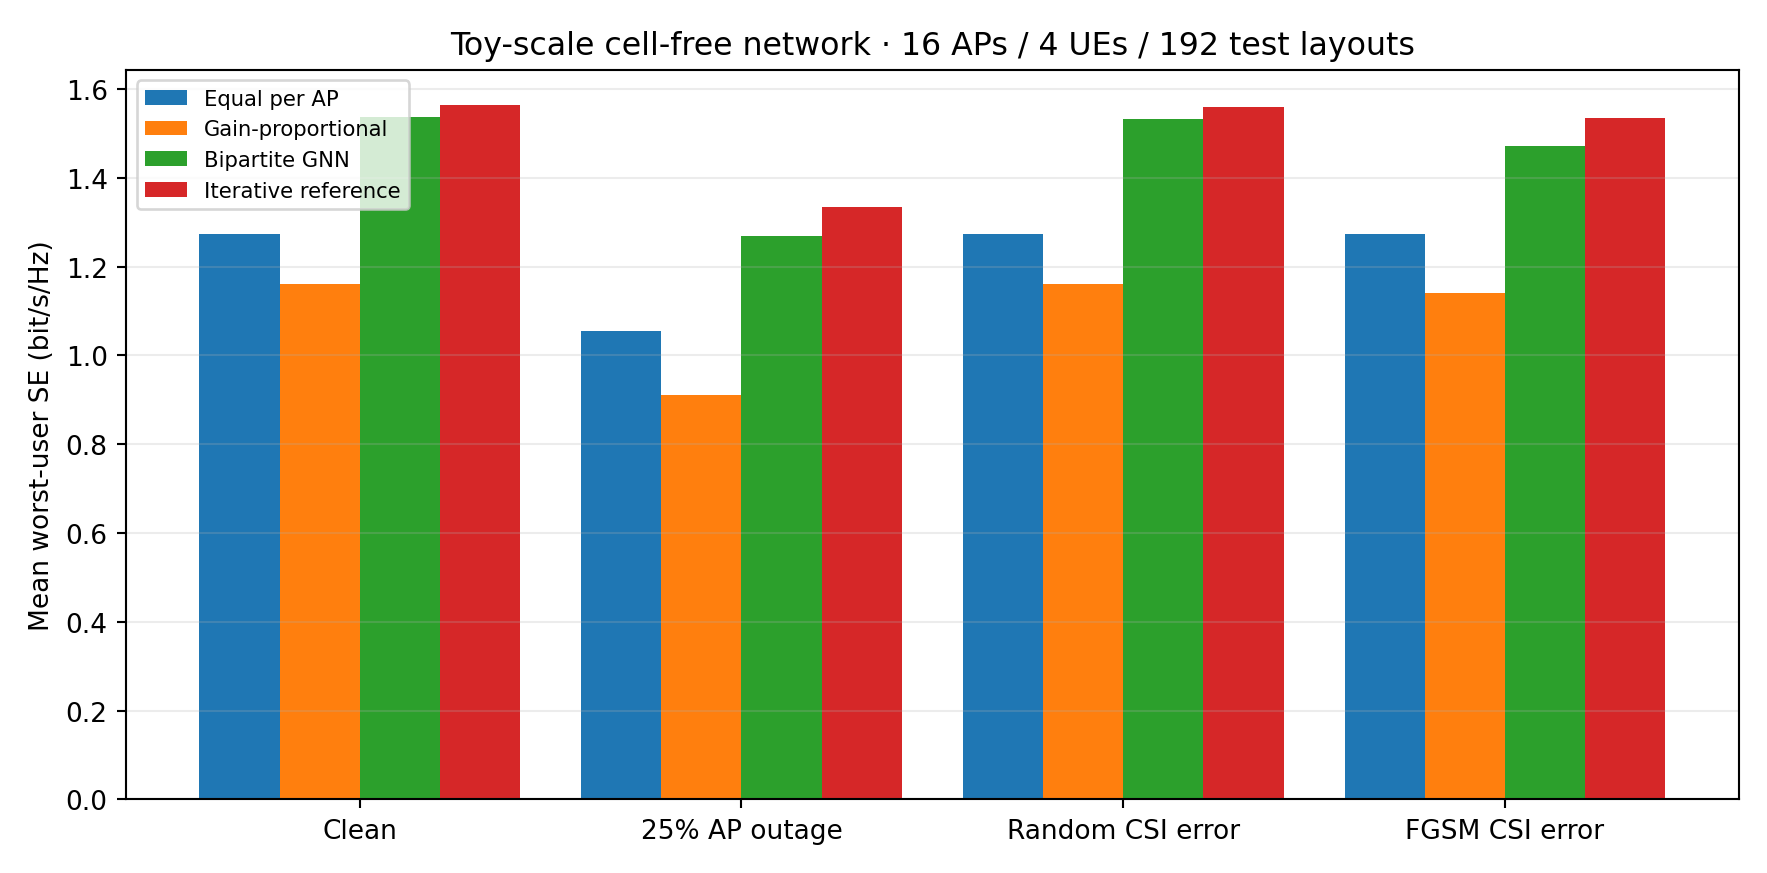
\includegraphics[width=.92\linewidth]{../figures/benchmark.png}
\caption{Worst-user rate across clean and stressed synthetic scenarios. The FGSM feature error is GNN-targeted.}\label{fig:results}
\end{figure}
\begin{figure}[H]\centering
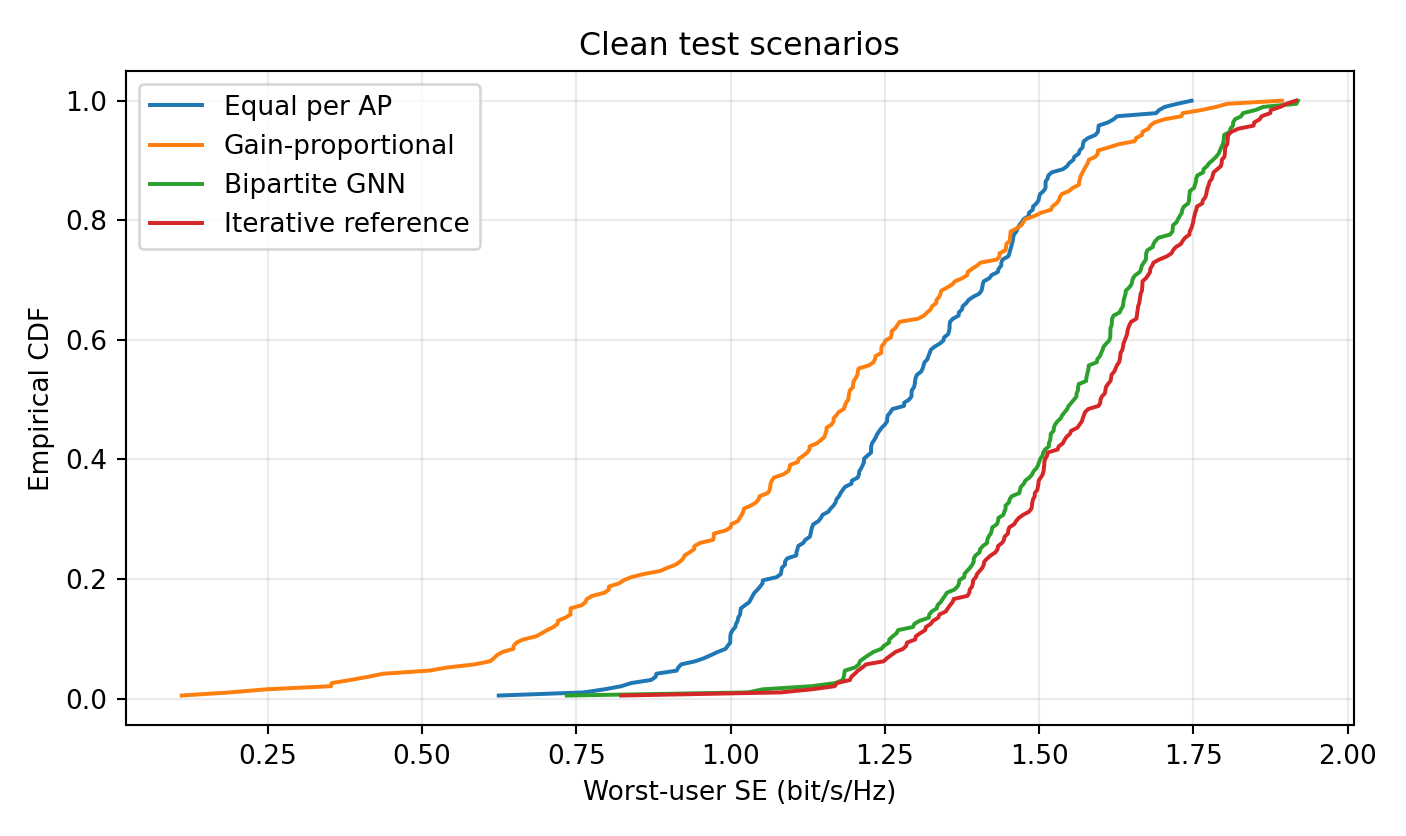
\includegraphics[width=.69\linewidth]{../figures/cdf_clean.png}
\caption{Empirical distribution of worst-user rate on the 192 clean test layouts.}\label{fig:cdf}
\end{figure}

\sect{Interpretation, validity and limitations}
The results are consistent with the usefulness of learning a graph-structured policy for fairness in this \emph{particular} stylized allocation problem. There is no proof of optimality, robustness certification, or new state-of-the-art result. The score of the baseline iterative procedure depends on its optimization budget, initialization, and smoothing temperature. Reported bootstrap intervals quantify scenario sampling variation \emph{conditional on one fixed training seed}; they do not account for model-training variability. Failing APs reduce available total transmit power, so the outage comparisons do not isolate controller robustness from physical capacity loss.

Important missing phenomena include pilot reuse and contamination, correlated fading, shadowing, mobility, calibrated 3GPP link budgets, practical fronthaul restrictions, finite coherence, unequal AP powers, control latency, imperfect association, multiple antennas per AP, and explicit hardware/energy constraints. We evaluate a \emph{single small system size}, not scaling or transfer across topologies. No denoising autoencoder, adversarial training, or PGD defense is implemented; those are future directions. Any internship or thesis extension should first add a stronger numerical max--min solver, multiple random training seeds, sensitivity to topology/association, and a realistic threat model.

\sect{Reproducibility and research-portfolio use}
The linked code repository includes a minimal installable package, dataset generator, training loop, saved GNN weights, seeds, scenario-level CSVs, metrics, figures, and unit tests for power feasibility and AP/UE permutation equivariance. From the repository root, run:
\begin{quote}\ttfamily\small
python -m pip install -e '.[dev]'\\
python -m pytest -q\\
python -m cfmimo.experiment --epochs 80 --train 480 --test 192 --seed 42\\
python -m cfmimo.plots
\end{quote}
Results were computed in Python/PyTorch on CPU. This independent study may be listed as \emph{``Research portfolio project (ongoing)''}, not as a peer-reviewed publication. Data are synthetically generated: no external private datasets or copyrighted IEEE article text are redistributed.

\begin{thebibliography}{9}\small
\bibitem{demir2021} \"O. T. Demir, E. Bj\"ornson and L. Sanguinetti, ``Foundations of User-Centric Cell-Free Massive MIMO,'' \emph{Foundations and Trends in Signal Processing}, 2021. \url{https://arxiv.org/abs/2108.02541}.
\bibitem{mishra2024} S. Mishra, L. Sala\"un, H. Yang and C. S. Chen, ``Graph Neural Network Aided Power Control in Partially Connected Cell-Free Massive MIMO,'' \emph{IEEE Trans. Wireless Commun.}, vol. 23, no. 9, pp. 12412--12423, 2024. DOI: \href{https://doi.org/10.1109/TWC.2024.3392441}{10.1109/TWC.2024.3392441}.
\bibitem{raghunath2024} R. Raghunath, B. Peng and E. A. Jorswieck, ``Energy-Efficient Power Allocation in Cell-Free Massive MIMO via Graph Neural Networks,'' 2024. \url{https://arxiv.org/abs/2401.14281}.
\bibitem{lin2025} ``Distributed Graph Neural Network Design for Sum Ergodic Spectral Efficiency Maximization in Cell-Free Massive MIMO,'' \emph{IEEE Trans. Veh. Technol.}, 2025. DOI: \href{https://doi.org/10.1109/TVT.2024.3493235}{10.1109/TVT.2024.3493235}.
\end{thebibliography}
\end{document}
